\documentclass{standalone}%
\usepackage[T1]{fontenc}%
\usepackage[utf8]{inputenc}%
\usepackage{lmodern}%
\usepackage{textcomp}%
\usepackage{lastpage}%
\usepackage{tikz}%
\usepackage{pgfplots}%
\pgfplotsset{compat=newest}%
%
\usetikzlibrary{positioning}%
%
\begin{document}%
\normalsize%
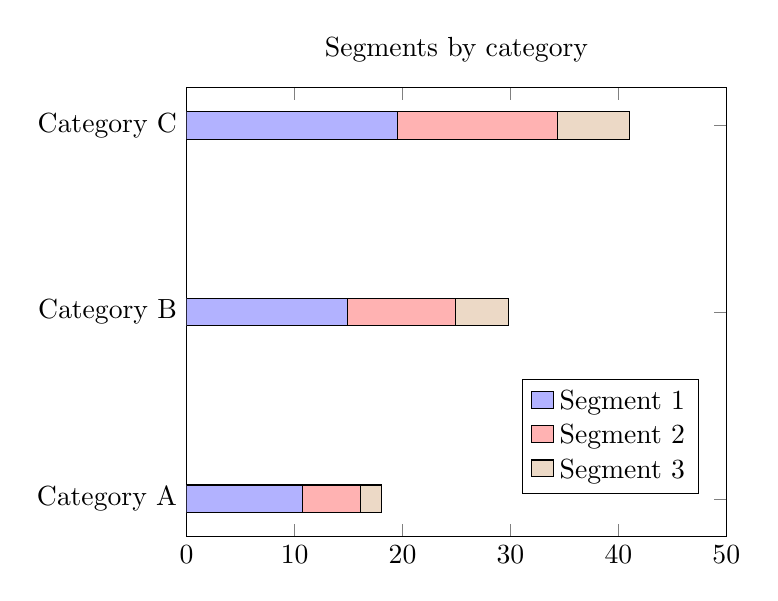
\begin{tikzpicture}%
\definecolor{color1}{RGB}{178, 178, 255}%
\definecolor{color2}{RGB}{255, 178, 178}%
\definecolor{color3}{RGB}{236, 217, 198}%
\begin{axis}[xbar stacked, name=barchart, title=Segments by category
, symbolic y coords={{Category A}, {Category B}, {Category C}}, ytick=data, legend style={at={(0.95, 0.35)}}, legend cell align={left}, xmin=0, xmax=50]%
\addplot[fill=color1] coordinates {%
(19.51,Category C)%
(14.88,Category B)%
(10.7,Category A)%
};%
%
%
\addplot[fill=color2] coordinates {%
(14.81,Category C)%
(10.06,Category B)%
(5.42,Category A)%
};%
%
%
\addplot[fill=color3] coordinates {%
(6.71,Category C)%
(4.88,Category B)%
(1.94,Category A)%
};%
%
%
\legend{Segment 1, Segment 2, Segment 3}%
\end{axis}%
\end{tikzpicture}%
\end{document}